\documentclass[handout, 9pt]{beamer}

%!TEX root = ../notas_de_clase.tex

%preamble

%language
\usepackage[spanish,es-nodecimaldot]{babel}
\usepackage[utf8]{inputenc}
\usepackage{apacite}
\usepackage[absolute,overlay]{textpos}

%packages
\usepackage[Algoritmo]{algorithm}
\usepackage{algorithmicx}
\usepackage[noend]{algpseudocode}
\usepackage{mathtools}
\setlength {\marginparwidth}{2cm}
\usepackage{todonotes}
\usepackage{amsbsy}
\usepackage{amssymb}
\usepackage{amsmath,bm}
\usepackage{dsfont}

\usepackage{xcolor}
\providecommand{\sred}[1]{\textcolor{red}{#1}}
\providecommand{\sblue}[1]{\textcolor{blue}{#1}}
\providecommand{\red}[1]{\textcolor{red}{\text{#1}}}
\providecommand{\blue}[1]{\textcolor{blue}{\text{#1}}}
\providecommand{\redb}[1]{\textcolor{red}{\textbf{#1}}}
\providecommand{\blueb}[1]{\textcolor{blue}{\textbf{#1}}}
\usepackage{graphicx}
\usepackage{fancybox}
\usepackage{booktabs}
\usepackage{caption}
\usepackage{float}
%\usepackage[longend,ruled,algochapter,linesnumbered,lined,boxed,commentsnumbered,spanish]{algorithm2e}
%\usepackage[algo2e]{algorithm2e}
\usepackage{amssymb}
\usepackage{amstext}
\usepackage{bm}
\usepackage{wrapfig}
\usepackage{subcaption} % para_unsupervised_chapter

%formatting

\usepackage[export]{adjustbox}

%caption para figuras
\captionsetup[figure]{width=.8\linewidth, font=small,labelfont={bf},name={Fig.},labelsep=period}
\captionsetup[table]{width=.8\linewidth,font=small,labelfont={bf},name={Tabla},labelsep=period}



\ifx\byn\undefined
    \definecolor{my_blue}{HTML}{C2D5FF}
    \definecolor{my_red}{HTML}{FFC2C2}
    \definecolor{my_yellow}{HTML}{FFFFE0}
\else
    \definecolor{my_blue}{HTML}{FFFFFF}
    \definecolor{my_red}{HTML}{FFFFFF}
    \definecolor{my_yellow}{HTML}{FFFFFF}
\fi


\usepackage[framemethod=TikZ]{mdframed}
\mdfdefinestyle{discusion}{%
    %linecolor=black,
    %outerlinewidth=0pt,
    roundcorner=0pt,
    innertopmargin=5pt,
    innerbottommargin=5pt,
    innerrightmargin=20pt,
    innerleftmargin=20pt,
    backgroundcolor=my_blue}

\colorlet{Green}{green!90}


\mdfdefinestyle{ejemplo}{%
    %linecolor=black,
    %outerlinewidth=0pt,
    roundcorner=0pt,
    innertopmargin=5pt,
    innerbottommargin=5pt,
    innerrightmargin=20pt,
    innerleftmargin=20pt,
    backgroundcolor=my_yellow}


\mdfdefinestyle{pendiente}{%
    style = discusion, 
    backgroundcolor=my_red}


\RequirePackage{url}



%definitions
\def\td{{\text d}}
\def\cN{{\mathcal N}}
\def\cX{{\mathcal X}} 
\def\cC{{\mathcal C}} 
\def\N{{\mathbb N}}
\def\d{{\text d}}
\def\datos{{\mathcal D}}
\def\eye{{\mathbb I}}
\def\ssum{{\scriptstyle\sum}}
\def\bepsilon{{\bm \epsilon}}
\def\tx{\tilde{x}}
\def\tX{\tilde{X}}
\def\thetaMAP{\theta_\text{MAP}}
\newcommand{\gp}{\ensuremath{\mathcal{GP}}}
\newcommand{\pr}{\ensuremath{\mathbb{P}}}
\newcommand{\x}{\ensuremath{\mathbf{x}}}
\newcommand{\z}{\ensuremath{\mathbf{z}}}
\newcommand{\cvector}{\ensuremath{\mathbf{c}}}
\newcommand{\e}{\ensuremath{\mathbf{e}}}
\newcommand{\y}{\ensuremath{\mathbf{y}}}
\newcommand{\bx}{\ensuremath{\textcolor{blue}{X}}}
\newcommand{\by}{\ensuremath{\textcolor{blue}{Y}}}
\newcommand{\rx}{\ensuremath{\textcolor{red}{X_*}}}

\newcommand{\R}{\mathbb{R}}
\newcommand{\norm}[1]{\left\lVert#1\right\rVert}




\DeclareMathOperator*{\argmax}{arg\,max}
\DeclareMathOperator*{\argmin}{arg\,min}
\DeclareMathOperator{\E}{\mathbb{E}}
\DeclareMathOperator{\V}{\mathbb{V}}
\DeclareMathOperator{\KL}{\text{KL}}
\DeclareMathOperator{\MVN}{\text{MVN}}
\newcommand\deq{\stackrel{\mathclap{\normalfont\mbox{\tiny def}}}{=}}
%\newcommand{\E}[1]{\mathbb E \left[#1\right]}
\newcommand{\trace}[1]{\text{Tr} \left[#1\right]}


\usepackage{amsthm}

%-------------------------------------------
% Newtheorem
%-------------------------------------------
\newtheorem{axioma}{\textcolor{red}{Axioma}}
\newtheorem{definicion}{Definición}
\newtheorem*{notacion}{Notación}
\newtheorem{teorema}{Teorema}
\newtheorem{corolario}{Corolario}
\newtheorem{lema}{Lema}
\newtheorem{lemaZ}{\textcolor{red}{Lema}}
\newtheorem{propiedad}{Propiedad:}
\newtheorem{proposicion}{Proposición:}
\newtheorem*{observacion}{Observación}
\newtheorem*{comentario}{Comentario}
\newtheorem*{ejemplo}{Ejemplo}
\newtheorem*{resultado}{Resultado}
\newtheorem*{propuesto}{Ejercicio propuesto}
\newtheorem*{demostracion}{Demostración} % No se usa, usar \begin{proof}\end{proof} que son por default.

%listing paackage para código
\usepackage{listings}
\usepackage{xcolor}
 
\definecolor{codegreen}{rgb}{0,0.6,0}
\definecolor{codegray}{rgb}{0.5,0.5,0.5}
\definecolor{codepurple}{rgb}{0.58,0,0.82}
\definecolor{backcolour}{rgb}{0.95,0.95,0.92}
 
\lstdefinestyle{mystyle}{
    xleftmargin=0.15\textwidth,
    linewidth=0.8\textwidth,
    backgroundcolor=\color{backcolour},   
    commentstyle=\color{codegreen},
    keywordstyle=\color{magenta},
    numberstyle=\tiny\color{codegray},
    stringstyle=\color{codepurple},
    basicstyle=\ttfamily\footnotesize,
    breakatwhitespace=true,         
    breaklines=true,                 
    captionpos=b,                    
    keepspaces=true,                 
    numbers=left,                    
    numbersep=5pt,                  
    showspaces=false,                
    showstringspaces=false,
    showtabs=false,                  
    tabsize=2
}
 
\lstset{style=mystyle}

\numberwithin{equation}{section}

\usetheme{simple}

\title{Clase 16: Clustering}
\subtitle{MA5204 Aprendizaje de Máquinas}
\date{\today}
\author{Felipe Tobar} 
\titlegraphic{
\begin{figure}[htp] 
    \centering
        
\includegraphics[width=0.15\textwidth]{../img/Uchile.pdf}% 
\end{figure}
}
\institute{Iniciativa de Datos e Inteligencia Artificial\\Universidad de Chile}

\begin{document}
\begin{frame}
  \titlepage
\end{frame}

%Clustering: idea general.
\begin{frame}{Clustering: idea general}
	
	Uno de los objtivos principales en el aprendizaje no supervisado es la agrupación de datos sin  etiquetas etiquetas (como ocurre en los métodos de clasificación).\\~\
	
	\pause
	La dificultad principal de esta tarea es que es necesario definir un concepto de \emph{similitud} 	entre las distintas entradas para poder particionar los datos en grupos (clusters) de características similares.
	
\end{frame}

%Hierarchical clustering (HCA).
\begin{frame}{Hierarchical clustering (HCA)}
	
	Corresponde al algoritmo de clustering más simple pero a su vez, es uno de los más caros computacionalmente. El objetivo es identificar $k$ clusters en los datos. \\~\ \pause

 El algoritmo aglomerativo de clustering es el siguiente:

\begin{enumerate}
	\item Para comenzar, se considerarán $n$ clusters distintos. Es decir, tantos cluster como datos y se asigna cada dato con un único cluster y viceversa.\pause
	\item Buscar el par de clusters más \emph{similar} (bajo algún criterio) y combinarlos en un solo cluster.\pause
	\item Repetir el paso anterior hasta tener $k$ clusters.
\end{enumerate}
\pause
Para dos clusters $A,B\subset\mathcal{D}$, los criterios de similitud más frecuentes son los siguientes:

\begin{itemize}
	\item \textbf{Single-linkage clustering:} $D_s(A,B):=\min\{d(a,b):a\in A, b\in B\}$.\pause
	\item \textbf{Complete-linkage clustering:} $D_s(A,B):=\max\{d(a,b):a\in A, b\in B\}$.\pause
	\item \textbf{Average-linkage clustering:} $D_a(A,B):=\frac{1}{|A|\cdot|B|}\sum_{a\in A, b\in B} d(a,b)$.\pause
\end{itemize}

Donde $d:\mathcal{D}\times \mathcal{D}\to \R_+$ es una métrica en $\mathcal{D}$. Elecciones distintas del criterio de similitud y/o métrica (generalmente euclidiana) pueden llevar a agrupaciones distintas.
	
\textbf{-->Lo anterior es el enfoque \emph{aglomerativo}, también hay otro \emph{divisivo}.}	
\end{frame}

%k-means.
\begin{frame}{$k$-means}

Otro método de clustering muy utilizado es $k$-means. Dado $k \in \mathbb{N}$ y un conjunto de observaciones $X = \{x_i\}_{i=1}$ con $x_i\in \mathbb{R}^D$ se busca separar los datos en $k$ grupos tal que:

\begin{itemize}
	\item Cada grupo se representa por un centroide $\mu_k$.\pause
	\item Cada elemento $x_i$ se asigna al grupo que tenga el centroide más \emph{cercano}.\pause
\end{itemize}

La asignación del dato $x_i$ al centroide $\mu_k$, denotada $r_{ik}$, está definida por:
\begin{align*}
r_{ik} = \begin{cases}
1 & \text{si } k = \text{argmin}||x_i-\mu_k||\\
0 & \text{si no.}
\end{cases}
\end{align*}

\pause
Es decir, para encontrar los centroides se debe minimizar el funcional:
\begin{align*}
J = \sum_{i=1}^N \sum_{k=1}^K r_{ik} ||x_i-\mu_k||^2.
\end{align*}
	
\end{frame}

%k-means: algoritmo de Lloyd.
\begin{frame}{$k$-means: algoritmo de Lloyd}
	El algoritmo más frecuente usado para k-means es el algoritmo de Lloyd:\pause

\begin{itemize}
    \item \textbf{E-step:} En este paso, se calculan (actualizan) las asignaciones $r_{ik}$, dejando fijas las medias $\mu_k$. Lo que corresponde a asignar el dato $x_i$ al centroide más cercano.\pause
    \item \textbf{M-step:} El siguiente paso corresponde a actualizar los centroides $\mu_k$ dejando fijas las asignaciones $r_{ik}$.\\~\
    \pause
    
    Como $J$ es cuadrática en $\mu_k$, entonces podemos utilizar la condición de primer orden:
    \begin{align*}
        \mu_k = \frac{\sum_{i=1}^N r_{ik}x_i}{\sum_{i=1}^N r_{ik}}.
    \end{align*}
    
    Lo que corresponde a asignar el centro del cluster al promedio de todas las muestras asignadas al antiguo cluster.
    \pause
    \item El algoritmo termina cuando los centroides ya no cambian.
\end{itemize}
\vspace{1em}
\textbf{--> ¿Por qué estas etapas se llama E y M?}

\end{frame}

%k-means: algoritmo de Lloyd.
\begin{frame}{$k$-means: algoritmo de Lloyd}
	Para los centroides iniciales, se tienen dos posibles inicializaciones:

\begin{itemize}
	\item \textbf{Método de Forgy:} se eligen de forma aleatoria $k$ puntos de la muestra como centroides iniciales.\pause
	\item \textbf{Random partition:} se eligen asignaciones aleatorias para los elementos. De este modo, los centroides iniciales serán los centroides obtenidos al realizar M-step.\pause
\end{itemize}

El método de Forgy es preferido cuando se realiza k-means mediante el algoritmo de Lloyd.\pause

\begin{figure}[h]
  \centering
  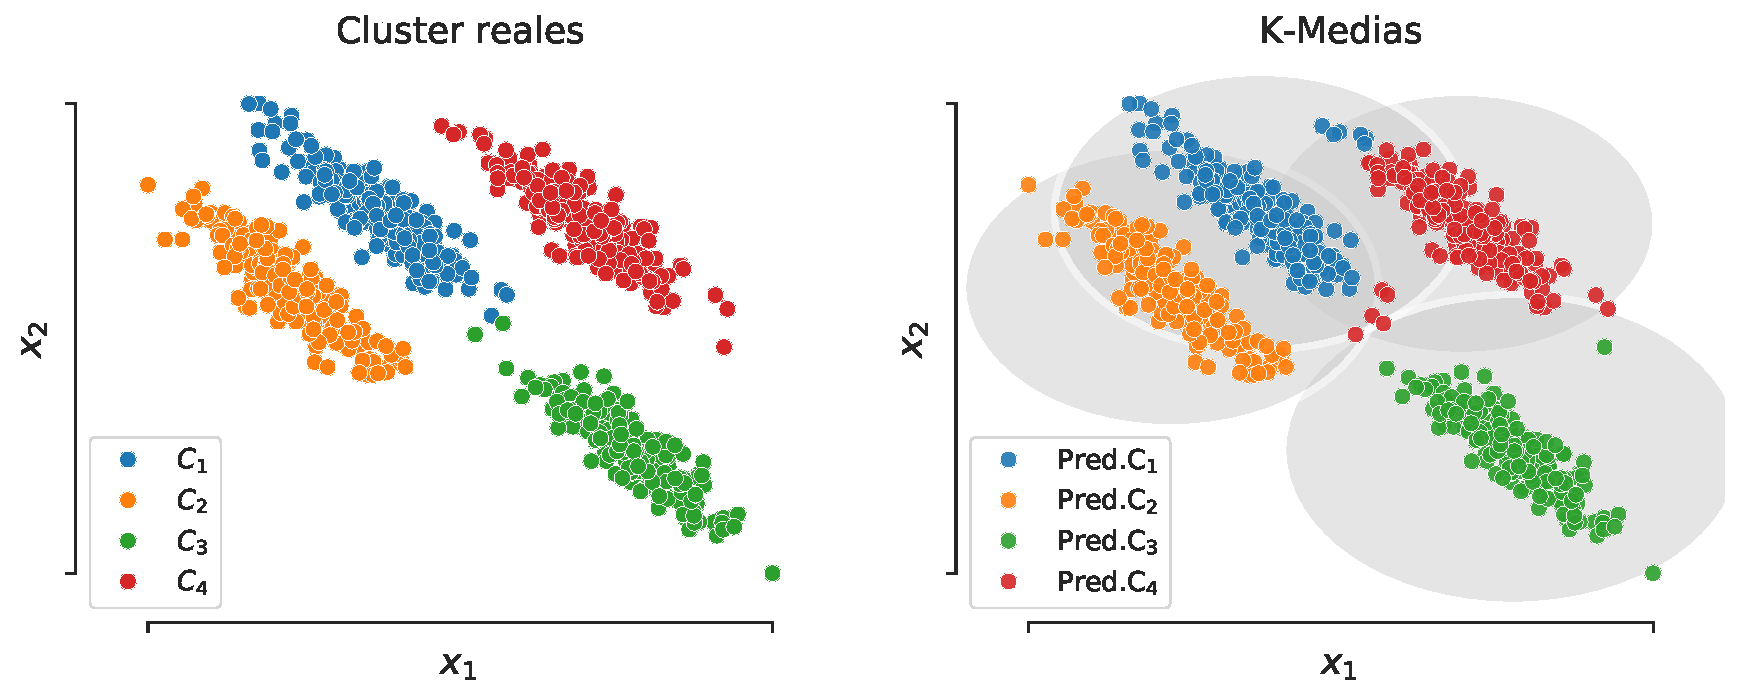
\includegraphics[width=0.7\textwidth]{../img/cap6_k_medias}
  \caption{Se observa que los clusters creados por kmeans son circulares, esto es debido a que se utiliza distancia euclidiana hace el centro del cluster.}
  \label{fig:kmeans}
\end{figure}

\end{frame}


%k-means: diagrama de Voronoi.
\begin{frame}{$k$-means: diagrama de Voronoi}
	
La asignación de cluster mediante el centroide más cecano provoca que cada par de centroides divida al espacio ambiente en dos semiespacios mediante el hiperplano simetral que pasa entre ambos puntos. \\~\ \pause

Dado que la intersección finita de semiespacios genera un poliedro, se tiene que la partición generada por $k$-means forma un diagrama de Voronoi:

\begin{figure}[h]
  \centering
  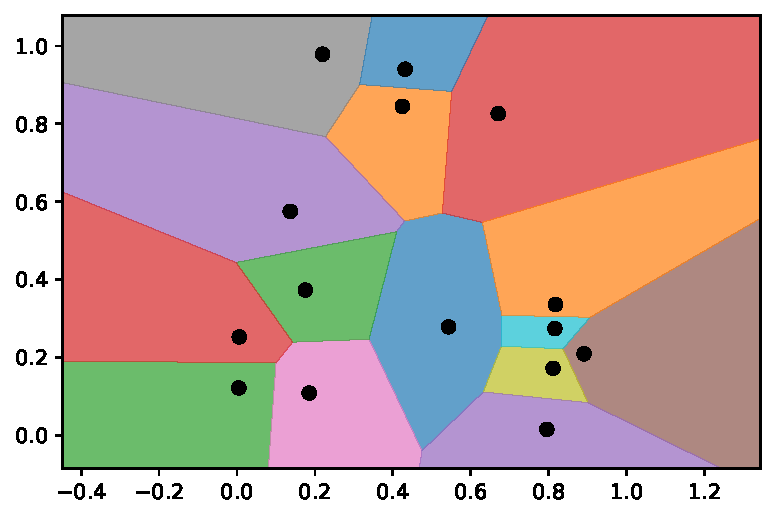
\includegraphics[width=0.5\textwidth]{../img/cap6_voronoi}
  \caption{Partición de $\mathbb{R}^2$ inducida por los centroides.}
  \label{fig:kmeans_voronoi}
\end{figure}

\end{frame}

%Modelo de mezcla de gaussianas (GMM)
\begin{frame}{Modelo de mezcla de gaussianas (GMM)}

La mezcla de gaussianas (GMM) es un caso general de $k$-means, en donde los clusters pueden tener una forma anisotrópica modelada por una Gaussiana. Si bien su solución puede ser muy similar a $k$-means los supuestos subyacentes al modelo GMM son diferentes y obedecen a un enfoque de modelo generativo. \\~\ \pause

Una distribución de mezcla de gaussianas consiste en una combinación convexa de distribuciones gaussianas
\begin{equation*}
	p(\x) = \sum_{k=1}^K \pi_k \mathcal{N}(\x| \mu_k,\Sigma_k),
\end{equation*}
donde $\sum_{k=1}^K \pi_k = 1$. \\~\

Una muestra $x$ es generada mediante dos etapas: primero se elige un cluster al azar (de acuerdo a $\pi_k$) y luego, se genera una muestra aleatoria dentro del cluster. \pause Nos referiremos a los parámetros de este modelo como 

\begin{itemize}
	\item $\pi_k:$ coeficiente de mezcla del cluster  $k$ (probabilidad de venir del cluster $k$).
	\item $\mu_k:$ media del cluster  $k$.
	\item $\Sigma_k:$ matriz de covarianza del cluster  $k$.
\end{itemize}

\end{frame}



%Modelo de mezcla de gaussianas (GMM): MV.
\begin{frame}{Modelo de mezcla de gaussianas (GMM): MV}
	
 La log-verosimilitud del modelo está dada por 

\begin{equation*}
	\log p(\x_1,\ldots,\x_N) = \sum_{n=1}^N \log p(\x_n) = \sum_{n=1}^N \log \sum_{k=1}^K  \pi_k\cN(\x_n|\mu_k,\Sigma_k) \label{eq:GMM_like}	
\end{equation*}\pause
Hay una serie de complicaciones relacionadas a la búsqueda de estos parámetros mediante MV:

\begin{itemize}
	\item \textbf{Singularidades:} cuando una muestra es exactamente igual a una de las medias, en cuyo caso un término de la log-verosimilitud es proporcional a $1/\sigma_k$, con lo que la maximización de $\sigma_k$ resulta en una log-verosimilitud infinita.\pause
	\item \textbf{Redundancias de soluciones:} para cada máximo local de la log-verosimilitd existen $k!$ soluciones equivalente con la misma verosimilitud dadas por las permutaciones de las etiquetas de los clusters.\pause
	\item \textbf{Funcional complejo:} la sumatoria aparece \emph{dentro} del logaritmo, consecuentemente, el logaritmo no actúa directamente en la gaussiana reduciendo el funcional de optimización a una solución en forma cerrada (caso cuadrático).
\end{itemize}

Este último problema obliga a considerar métodos basados en gradientes.

\end{frame}


%Modelo de mezcla de gaussianas (GMM): entrenamiento.
\begin{frame}{Modelo de mezcla de gaussianas (GMM): entrenamiento}
	
Veamos las condiciones de primer orden sobre la log-verosimilitud para encontrar los parámetros.\\~\

Denotando $\gamma(z_k(\x_i)) = p(z_k(\x_i)=1|\x_i)$, se tiene el siguiente resultado:

\begin{lemma} Para el modelo GMM, los parámetros óptimos son
	\begin{align*}
    \mu_k & = \frac{1}{R_k}\sum_{i=1}^N \gamma(z_k(\x_i))\x_i\\
    \Sigma_k & = \frac{1}{R_k} \sum_{i=1}^N \gamma(z_k(\x_i))(\x_n - \mu_k)(\x_n - \mu_k)^\top\\
    \pi_k & = \frac{R_k}{R},
    \end{align*}
    donde $R_k = \sum\limits_{i=n}^N \gamma(z_k(\x_i))$ y $R = \sum\limits_{k=1}^K R_k$.
\end{lemma}
	
\end{frame}


\begin{frame}
Esto no constituye una solución en forma cerrada para los parámetros ya que la posterior $\gamma(z_k(\x_i))$ depende de todos los parámetros:
\begin{align*}
	p(z_k(\x)=1|\x) = \frac{p(\x|z_k(\x)=1)p(z_k(\x)=1)}{p(\x)} = \frac{\pi_k \cN(\x|\mu_k,\Sigma_k)}{\sum_{k=1}^K \pi_k \cN(\x|\mu_k,\Sigma_k)} .
\end{align*} 
\pause

Sin embargo, podemos considerar un procedimiento iterativo en donde calculamos las posteriores $\gamma(z_k(\x_i))$ (llamado paso E), para luego calcular los parámetros óptimos de acuerdo a las ecuaciones anteriores (llamado paso M). \pause

\begin{figure}[ht]
  \centering
  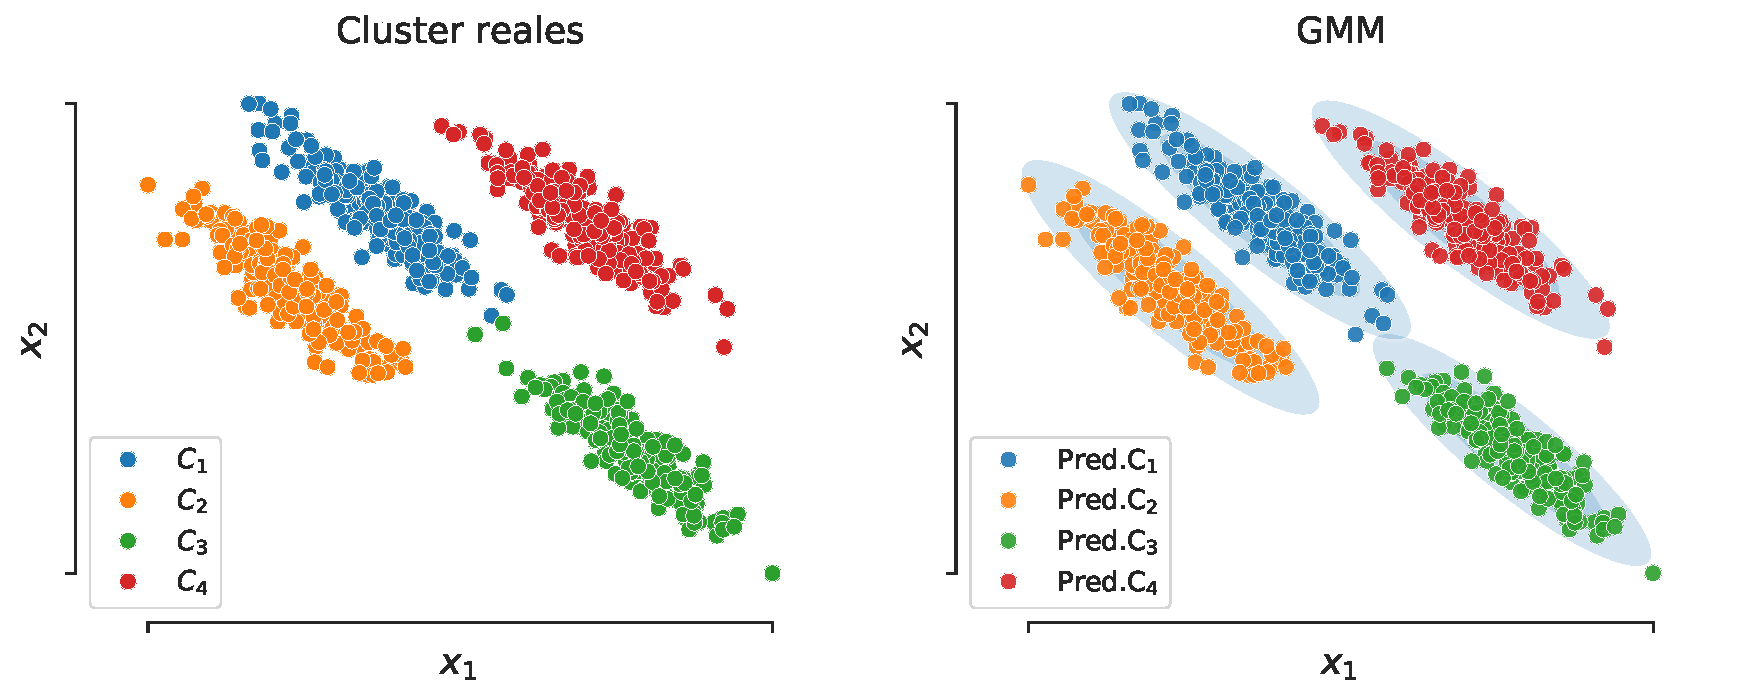
\includegraphics[width=0.7\textwidth]{../img/cap6_gmm}
  \caption{Se observa como GMM es una generalización de $k$-means, donde ahora los clusters tienen forma de gaussiana anisotrópica.}
  \label{fig:gmm}
\end{figure}

\end{frame}


\end{document}
